% \vspace{-\baselineskip}

%-------------------------------------------------------------------------------
\section{Introduction}
\label{sec:introduction}
%-------------------------------------------------------------------------------

For many, Internet Protocol~(IP) lookup is considered a challenge of the past. With over 40 years of research and hundreds of papers (e.g., ~\cite{dir, lulea, lampson, dxr, tree_bitmap, dharma, poptrie, hibst, sail}) focused on supporting IP lookup at scale, numerous schemes have been developed---some of which have been in practical use for two decades. However, these classical approaches are {\em single-resource} solutions, designed for conventional switch chip architectures that provided either specialized hardware like ternary content-addressable memory~(TCAM) or commodity random-access memory~(RAM), such as on-chip static RAM~(SRAM) coupled with off-chip dynamic RAM~(DRAM), but not both. TCAM enables parallel searches across wildcarded entries in a single clock cycle but requires three times more transistors per bit than SRAM and consumes hundreds of watts~\cite{tcampower}. RAM-based approaches are cheaper but require additional complexity and memory compared to pure TCAM solutions. Thus far, commercial switch chip vendors have scaled these {\em single-resource} solutions by increasing hardware resources.

In this paper, we contend that it is important to reconsider IP lookup due to the continued growth of lookup tables and a recent inflection point in network hardware. A slew of new application-specific integrated circuits~(ASICs), such as Intel Tofino~\cite{intel_tofino}, AMD Pensando~\cite{amd_pensando}, and Nvidia BlueField~\cite{nvidia_bluefield}, have transformed the networking chip market~\cite{p4_ecosystem}. These chips are built on two modern packet processing architectures---Reconfigurable Match-Action Tables~(RMT)\cite{rmt} and disaggregated RMT~(dRMT)\cite{drmt}---which consist of match-action processors with access to large amounts of {\em both} TCAM and SRAM. We review these architectures at the start of \cref{sec:cram}. This leads us to our central question: \textit{How can we leverage modern networking chips, utilizing both TCAM and SRAM, to develop new IP lookup algorithms that scale to larger databases than classical single-resource solutions?}

Two main challenges make designing scalable algorithms for RMT and dRMT chips difficult:
\begin{inlist}
  \item Lack of an abstract model for evaluating and comparing algorithms. Chip-specific arcana such as memory allocation, metadata storage, and action bits must be carefully considered.
  \item Large but finite resources. While TCAM, SRAM, and pipeline stages are available in substantial amounts, they require careful algorithm design to scale effectively.
\end{inlist}

\textbf{Solution}: We introduce the \cram~(CAM+RAM) lens, an abstract model of modern packet processing architectures, such as RMT and dRMT, paired with a set of optimization idioms. The \cram model enables us to estimate algorithm scalability using higher-order space and time metrics, without requiring simulation of ASIC-specific details such as TCAM block sizes, SRAM page sizes, and per-stage memory. The \cram model goes beyond classical models such as random-access machine~(RAM)~\cite{ram} and parallel RAM~(PRAM)~\cite{pram} by adding TCAM operations and using match-action dependencies to measure time complexity. The optimization idioms provide eight strategies for designing scalable algorithms.

%While 
\cram can be generalized to other hardware architectures, such as %manycore 
smart network interface cards~(SmartNICs)~\cite{intel_ipu, amd_pensando, nvidia_bluefield} and field-programmable gate arrays~(FPGAs)~\cite{intel_fpga, amd_fpga}, and applied to broader network applications like packet classification~\cite{pkt_class_surv1, pkt_class_surv2, pkt_class_surv3} and in-network machine learning~(ML)~\cite{homunculus, planter, inml_survey}. However, this is not the focus of our paper. For completeness, we briefly discuss these extensions in \cref{subsec:other_architectures} and \cref{subsec:other_applications}. Instead, we concentrate on applying \cram to {\em IP lookup} because of the following observations:

\begin{figure}[!t]
    \centering
    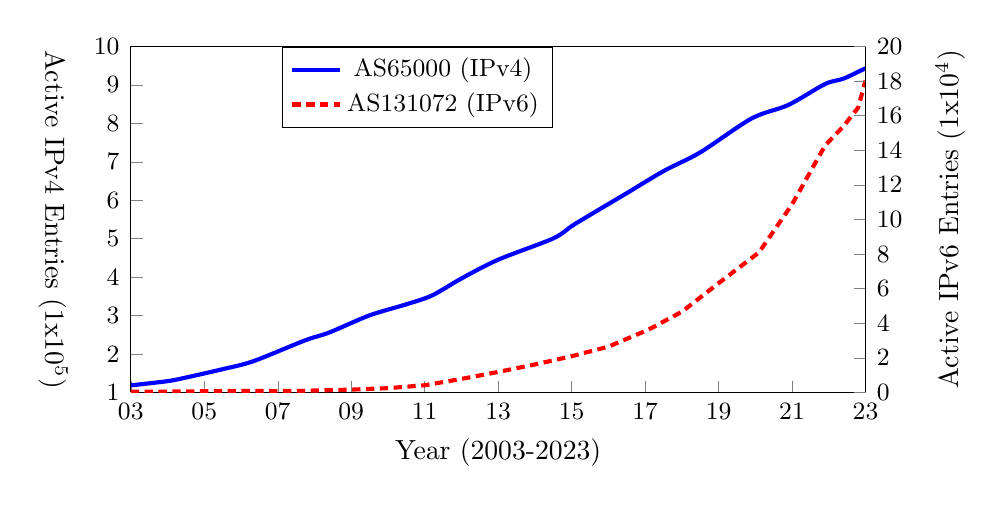
\begin{tikzpicture}
    \large
    \begin{axis}[
        xmin = 3, xmax = 23,
        ymin = 1, ymax = 10,
        xtick={3,5,...,23},
        ytick={1,2,...,10},
        axis y line* = left,
        width=\columnwidth*0.9,
        height=170pt,
        xticklabel={\ifdim\tick pt<10pt 0\fi\pgfmathprintnumber{\tick}},
        xticklabel style={rotate=0,font=\small},
        yticklabel style={rotate=0,font=\small},
        xlabel style={font=\normalsize,at={(axis description cs:.5,-.1)}},
        ylabel style={font=\normalsize,at={(axis description cs:-.07,.5)}},
        legend style={at={(0.575,1)},anchor=north east,font=\small},
        xlabel=Year (2003-2023),
        ylabel=Active IPv4 Entries (1x$10^5$),
        tick pos=left
    ]
    \addplot[line width=1.5pt,mark=none,smooth,color=blue]
        coordinates{
            (3,1.18362)
            (4,1.29296)
            (4.5,1.38674)
            (5.5,1.60471)
            (6.33,1.81032)
            (7.75,2.35660)
            (8.4,2.55837)
            (9.5,3.00500)
            (10.5,3.29240)
            (11.2,3.52301)
            (12,3.96490)
            (13,4.45339)
            (14.5,5.00789)
            (15.1,5.38775)
            (16.5,6.18431)
            (17.5,6.75741)
            (18.5,7.24538)
            (19.9,8.12839)
            (20.9,8.47974)
            (21.9,9.02461)
            (22.4,9.16372)
            (23,9.43586)
        };
    \addlegendentry{AS65000 (IPv4)}
    \addplot[line width=1.5pt,mark=none,densely dashed,color=red]
        coordinates{
            (-100,-100)
        };
    \addlegendentry{AS131072 (IPv6)}
    \end{axis}
    \begin{axis}[
        xmin = 3, xmax = 23,
        ymin = 0, ymax = 20,
        hide x axis,
        hide y axis,
        width=\columnwidth*0.9,
        height=170pt
    ]
    \addplot[line width=1.5pt,mark=none,densely dashed,color=red]
        coordinates{
            (3,0.0405)
            (4,0.05)
            (5,0.0706)
            (6,0.0853)
            (7,0.0793)
            (7.7,0.0918)
            (8,0.113)
            (9,0.1632)
            (10,0.2485)
            (11,0.4158)
            (12,0.7828)
            (13,1.1867)
            (14,1.6179)
            (15,2.0955)
            (16,2.6476)
            (17.1,3.6395)
            (18,4.6645)
            (19,6.3162)
            (20.1,8.0989)
            (21,10.8725)
            (21.9,14.2827)
            (22.4,15.3904)
            (22.8,16.4702)
            (23,18.0344)
        };
    \end{axis}
    \pgfplotsset{every axis y label/.append style={rotate=180}}
    \begin{axis}[
        xmin=0, xmax=1,
        ymin=0, ymax=20,
        hide x axis,
        axis y line*=right,
        ylabel=Active IPv6 Entries (1x$10^4$),
        ytick={0,2,...,20},
        width=\columnwidth*0.9,
        height=170pt,
        yticklabel style={rotate=0,font=\small},
        ylabel style={font=\normalsize,at={(axis description cs:1.08,.5)}}
    ]
    \end{axis}
    \end{tikzpicture}
    \vspace{-1em}
    \caption{BGP routing table size over the past two decades}
    \label{fig:bgp_growth}
    \vspace{-\baselineskip}
\end{figure}

{\bf O1. Continued IPv4 growth:} Over the past two decades, the global IPv4 routing table has grown {\em linearly}~\cite{cidr_report_ipv4, bgp_report_ipv4}, doubling in size every decade (\cref{fig:bgp_growth}). If this trend continues, the IPv4 table could reach two million entries by 2033.

{\bf O2. Rapid IPv6 deployment:} In the same period, the global IPv6 routing table has grown {\em exponentially}~\cite{cidr_report_ipv6, bgp_report_ipv6}, doubling every three years (\cref{fig:bgp_growth}). Even if growth slows to a linear rate, the IPv6 table could still reach half a million entries by 2033. IPv6 prefixes are also four times wider, though typically, only the first 64 bits are used for global routing.

{\bf O3. Virtual private networks~(VPNs):} Some routers maintain hundreds of VPN routing tables. On such devices, publicly available routing tables account for only a fraction of the total capacity required.

{\bf O4. Other tasks:} Routers need table memory for additional tasks such as network address translation~(NAT) and firewalls. Minimizing the memory used for forwarding allows more features to fit on a chip.

\cram enables us to rethink pre-existing IP lookup schemes, such as \sail~\cite{sail}, \dxr~\cite{dxr}, and multibit tries, to develop new algorithms that scale to larger databases. We start with the best-of-breed algorithms from three classic IP lookup approaches---search on prefix {\em lengths}, search on prefix {\em ranges}, and trie-based search. We derive new algorithms using the optimization idioms~(\cref{subsec:optimization_idioms}) and predict their scalability with the \cram model~(\cref{subsec:cram_model}). Each new algorithm---rethinking \sail~(\resail), Binary Search with Initial CAM~(\bsic), and \mashup---offers unique strengths for different settings.

We chose Intel Tofino-2, an RMT switch chip, for our experiments because we had access to its development environment. While Intel recently announced it will not develop new Tofino models, it remains committed to supporting Tofino and Tofino-2~\cite{nick_letter}. We expect our results to hold for dRMT, as RMT is a stricter version of dRMT with additional access restrictions.



This paper makes the following contributions:

\textbf{1. IP Lookup Algorithms:} Three new scalable IP lookup algorithms---\resail, \bsic, and \mashup.

\textbf{2. \cram Model:} An abstract model for quickly estimating the scalability of packet processing algorithms before detailed implementation.

\textbf{3. Optimization Idioms:} Eight design strategies for minimizing TCAM, SRAM, and pipeline stages.

\textbf{4. Evaluation:} Simulations and Tofino-2 implementations achieve 9X (IPv4) and 3X (IPv6) improvements over pure TCAM solutions, enabling scalability for the next decade.

The remainder of this paper is organized as follows. \cref{sec:cram} introduces the \cram model and optimization idioms, followed by an overview of the idioms in action. It also briefly explores other hardware architectures, broader network applications, and algorithmic requirements. We design three new IP lookup algorithms in \cref{sec:resail}, \cref{sec:bsic}, and \cref{sec:mashup}. \cref{sec:results} presents simulation and implementation results, followed by scalability experiments in \cref{sec:scalability}. \cref{sec:crammodelevaluation} evaluates the predictive accuracy of the \cram model, and \cref{sec:related} surveys related work. We conclude in \cref{sec:conclusion}.